\section{Raw data audit}

\subsection{Dataset overview}

The raw dataset contains 7043 observations and 21 columns. No exact duplicate rows were found, and pandas did not detect any standard missing values.

\begin{table}[H]
\centering
\caption{Raw dataset overview}
\begin{tabular}{lr}
\toprule
Item & Value \\
\midrule
Number of rows & 7043 \\
Number of columns & 21 \\
Duplicate rows & 0 \\
Total standard missing values & 0 \\
Columns with standard missing values & 0 \\
\bottomrule
\end{tabular}
\end{table}

The absence of standard missing values does not automatically imply that the dataset contains no missing information. A separate check for disguised missing values is still needed, especially for string columns where blanks or placeholder strings can hide missingness.

\subsection{Target distribution}

Table \ref{tab:target-distribution} shows the target distribution in the raw data. The dataset is moderately imbalanced: approximately 26.5\% of customers churned.

\begin{table}[H]
\centering
\caption{Target distribution in the raw dataset}
\label{tab:target-distribution}
\begin{tabular}{lrr}
\toprule
Target level & Count & Percentage \\
\midrule
No & 5174 & 73.46 \\
Yes & 1869 & 26.54 \\
\bottomrule
\end{tabular}
\end{table}

The imbalance is not extreme, but it is large enough that accuracy alone will not be sufficient for later model evaluation. Later modelling sections should include metrics that distinguish false positives from false negatives, such as precision, recall, F1-score, ROC-AUC, PR-AUC, and confusion matrices.

\subsection{Identifier check}

The column \texttt{customerID} has 7043 unique values for 7043 rows. It is therefore a unique identifier candidate. This is a raw-data fact. The modelling decision is to exclude it from the predictive feature set, because a unique identifier does not provide a generalizable customer characteristic.

\begin{table}[H]
\centering
\caption{Identifier check}
\begin{tabular}{lrrr}
\toprule
Column & Unique values & Number of rows & Unique value ratio \\
\midrule
customerID & 7043 & 7043 & 1.00 \\
TotalCharges & 6531 & 7043 & 0.93 \\
MonthlyCharges & 1585 & 7043 & 0.23 \\
tenure & 73 & 7043 & 0.01 \\
\bottomrule
\end{tabular}
\end{table}

\subsection{Disguised missing values in \texttt{TotalCharges}}

Although pandas detected no standard missing values, the string-column audit found 11 blank strings in \texttt{TotalCharges}. This is important because \texttt{TotalCharges} is conceptually numeric, but the blank strings caused it to be loaded as a string-like column.

\begin{table}[H]
\centering
\caption{Blank-string audit}
\begin{tabular}{lrrr}
\toprule
Column & Blank string count & Blank string percentage & Unique values \\
\midrule
TotalCharges & 11 & 0.16 & 6531 \\
customerID & 0 & 0.00 & 7043 \\
PaymentMethod & 0 & 0.00 & 4 \\
MultipleLines & 0 & 0.00 & 3 \\
InternetService & 0 & 0.00 & 3 \\
\bottomrule
\end{tabular}
\end{table}

The blank values in \texttt{TotalCharges} were then checked against \texttt{tenure}. The result is exact: the 11 blank \texttt{TotalCharges} rows are exactly the 11 rows where \texttt{tenure = 0}.

\begin{table}[H]
\centering
\caption{Relationship between blank \texttt{TotalCharges} and zero tenure}
\begin{tabular}{lr}
\toprule
Condition & Count \\
\midrule
Blank \texttt{TotalCharges} & 11 \\
\texttt{tenure == 0} & 11 \\
Blank \texttt{TotalCharges} and \texttt{tenure == 0} & 11 \\
Blank \texttt{TotalCharges} and \texttt{tenure != 0} & 0 \\
Non-blank \texttt{TotalCharges} and \texttt{tenure == 0} & 0 \\
\bottomrule
\end{tabular}
\end{table}

Converting \texttt{TotalCharges} to numeric creates exactly 11 missing values, which are the same blank strings:

\begin{table}[H]
\centering
\caption{\texttt{TotalCharges} numeric conversion check}
\begin{tabular}{lr}
\toprule
Item & Count \\
\midrule
Standard missing before conversion & 0 \\
Missing after numeric conversion & 11 \\
New missing created by numeric conversion & 11 \\
Blank string count & 11 \\
\bottomrule
\end{tabular}
\end{table}

\subsection{Inspection correction}

The raw dataset is preserved as \texttt{df\_raw}. A corrected inspection copy, \texttt{df\_inspect}, is created after the raw audit confirms the issue:

\begin{enumerate}[leftmargin=*]
    \item \texttt{TotalCharges} is converted from string to numeric.
    \item The 11 rows with \texttt{tenure = 0} and blank \texttt{TotalCharges} are set to \texttt{TotalCharges = 0.0}.
\end{enumerate}

This is justified because customers with zero tenure have not accumulated charges yet. This correction is applied before numeric summaries and visualizations, so the later inspection does not mistakenly treat \texttt{TotalCharges} as a categorical string variable.


\section{Feature summaries after inspection correction}

\subsection{Feature types}

After the inspection correction, the dataset has three numeric features:

\[
\texttt{tenure}, \quad \texttt{MonthlyCharges}, \quad \texttt{TotalCharges}.
\]

The remaining predictors are categorical or binary categorical. The feature \texttt{SeniorCitizen} is stored as an integer, but semantically it is a binary categorical feature.

\begin{table}[H]
\centering
\caption{Feature groups after inspection correction}
\begin{tabular}{lrp{9cm}}
\toprule
Feature group & Count & Features \\
\midrule
Numeric & 3 & tenure, MonthlyCharges, TotalCharges \\
Categorical or binary & 17 & gender, Partner, Dependents, PhoneService, MultipleLines, InternetService, OnlineSecurity, OnlineBackup, DeviceProtection, TechSupport, StreamingTV, StreamingMovies, Contract, PaperlessBilling, PaymentMethod, Churn, SeniorCitizen \\
\bottomrule
\end{tabular}
\end{table}

For later modelling, \texttt{Churn} is the target and is not part of the feature set.

\subsection{Numeric summary}

\begin{table}[H]
\centering
\caption{Numeric summary after inspection correction}
\begin{tabular}{lrrrrrrrr}
\toprule
Feature & Count & Mean & Std. & Min & 25\% & Median & 75\% & Max \\
\midrule
tenure & 7043 & 32.37 & 24.56 & 0.00 & 9.00 & 29.00 & 55.00 & 72.00 \\
MonthlyCharges & 7043 & 64.76 & 30.09 & 18.25 & 35.50 & 70.35 & 89.85 & 118.75 \\
TotalCharges & 7043 & 2279.73 & 2266.79 & 0.00 & 398.55 & 1394.55 & 3786.60 & 8684.80 \\
\bottomrule
\end{tabular}
\end{table}

\subsection{Categorical summary}

The categorical summary was used to check whether variables have sensible levels and whether any category dominates strongly. The most important example is \texttt{Contract}, where \texttt{Month-to-month} is the most common level at approximately 55.0\%.

\begin{table}[H]
\centering
\caption{Selected categorical feature summaries}
\begin{tabular}{lrlrr}
\toprule
Feature & Levels & Most common level & Most common count & Most common percentage \\
\midrule
PaymentMethod & 4 & Electronic check & 2365 & 33.58 \\
Contract & 3 & Month-to-month & 3875 & 55.02 \\
MultipleLines & 3 & No & 3390 & 48.13 \\
OnlineSecurity & 3 & No & 3498 & 49.67 \\
OnlineBackup & 3 & No & 3088 & 43.85 \\
\bottomrule
\end{tabular}
\end{table}

\section{Exploratory visual inspection}

\subsection{Why visual inspection is included}

Descriptive statistics alone can hide important patterns. The preprocessing lecture gives the example of Anscombe's quartet and the Datasaurus dozen to show that datasets can share similar summary statistics while having very different structures. Therefore, visual inspection is a necessary part of data understanding \cite{ml-preprocessing}. The goal here is not to select features manually, but to understand the shape and quality of the data before modelling.

\subsection{Numeric feature distributions}

Figure \ref{fig:numeric-distributions} shows histograms and boxplots for the three numeric features. \texttt{TotalCharges} is right-skewed, which is expected because accumulated charges increase over a customer's lifetime and many customers have relatively low accumulated charges. \texttt{tenure} has visible mass near very low tenure and near the upper end of the range.

\begin{figure}[H]
\centering

\includegraphics[width=\textwidth]{figures/numeric_feature_distributions.png}
\caption{Numeric feature distributions and boxplots}
\label{fig:numeric-distributions}
\end{figure}

No automatic outlier removal is performed at this stage. Extreme values should first be interpreted as either natural or unnatural outliers. The preprocessing lecture distinguishes unnatural outliers, such as coding or measurement errors, from natural extreme observations that may be part of the real production distribution \cite{ml-preprocessing}. Based on the plots, the numeric ranges appear plausible for this dataset, so no global outlier treatment is applied yet.

\subsection{Numeric correlation matrix}

Figure \ref{fig:numeric-correlation} shows the Pearson correlation matrix among numeric features and \texttt{Churn\_binary}. The target is included only as a simple linear association diagnostic.

\begin{figure}[H]
\centering
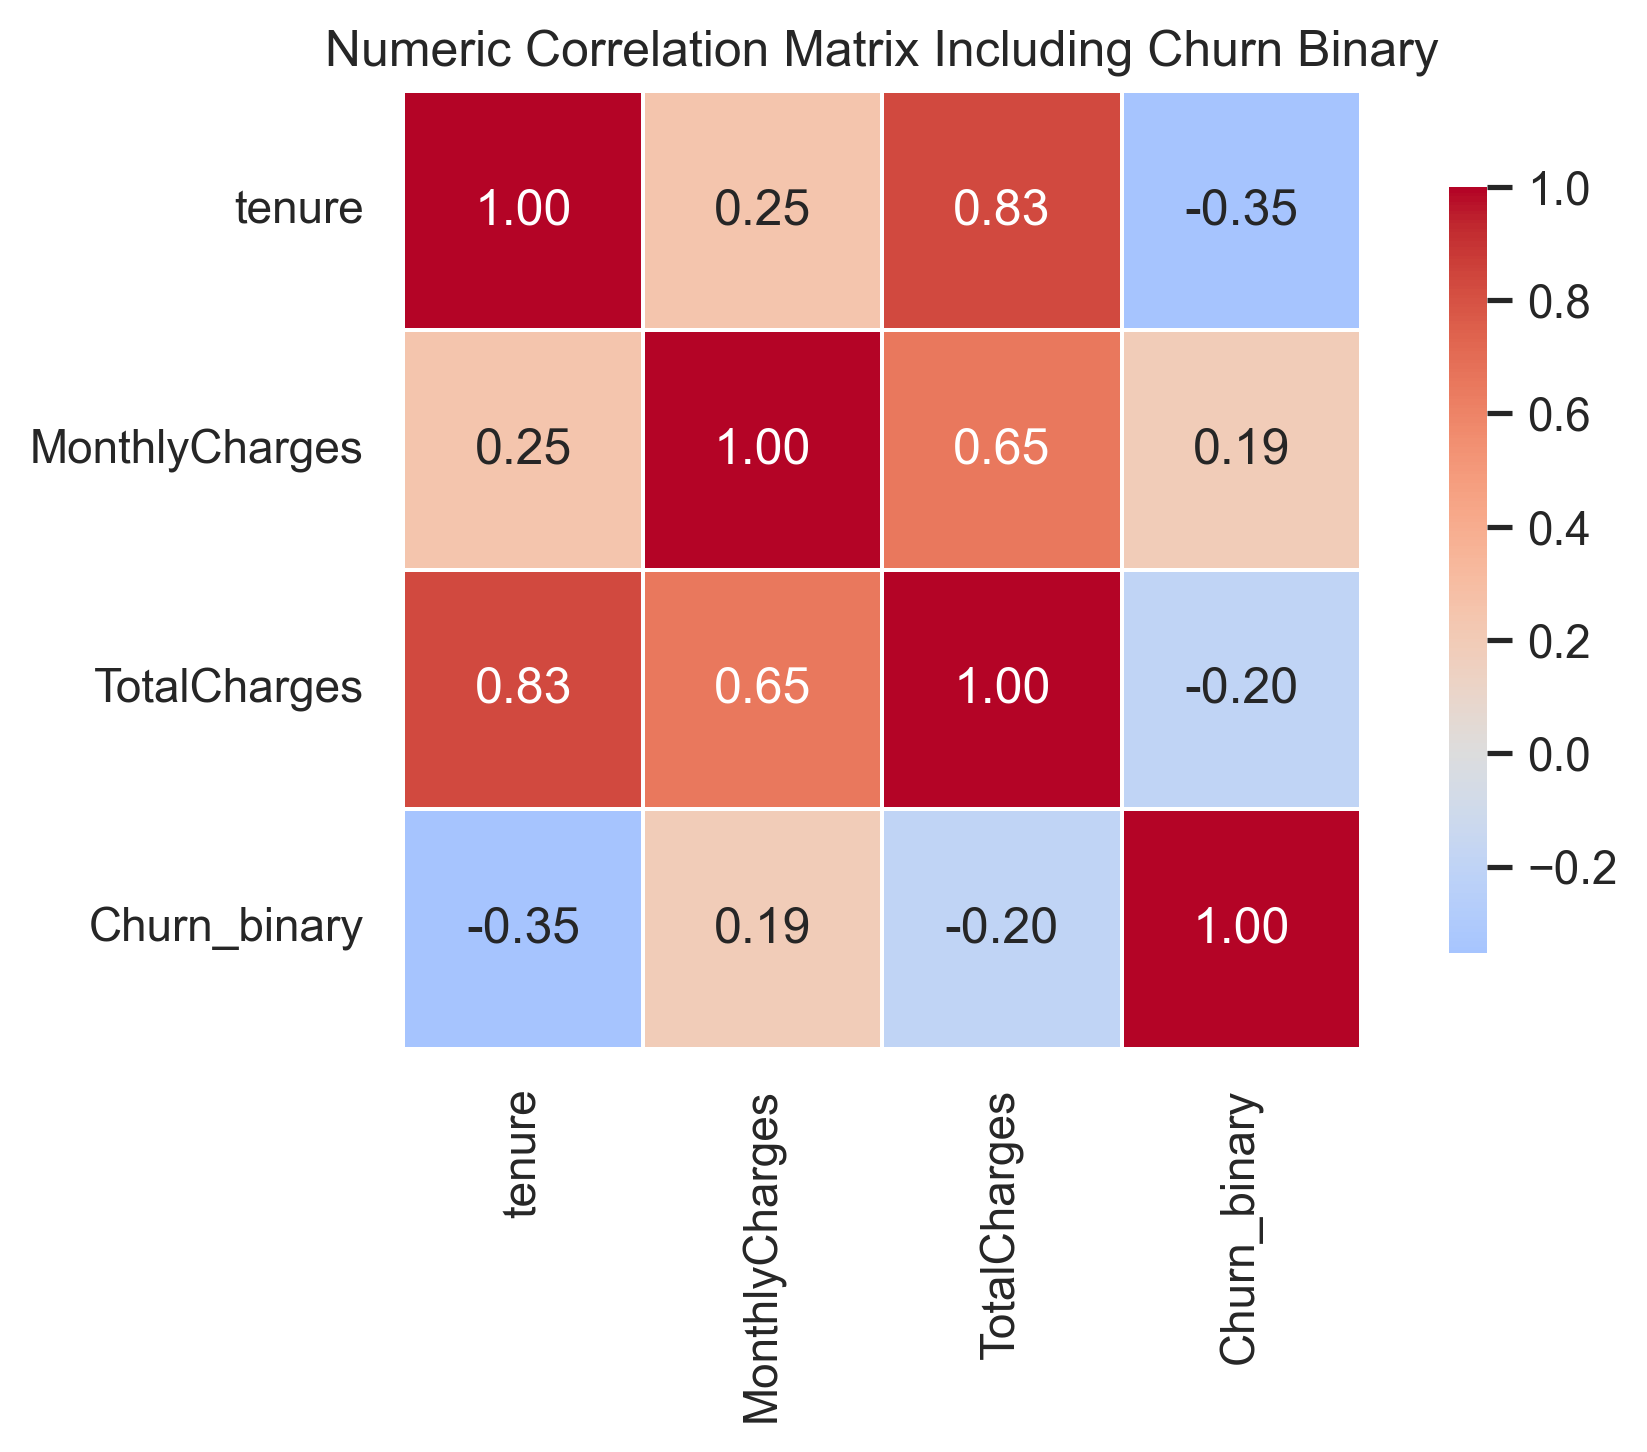
\includegraphics[width=0.78\textwidth]{figures/numeric_correlation_matrix.png}
\caption{Numeric correlation matrix including \texttt{Churn\_binary}}
\label{fig:numeric-correlation}
\end{figure}

The strongest numeric association is between \texttt{tenure} and \texttt{TotalCharges}, with correlation 0.83. This is expected because total charges accumulate over time. The strongest simple correlation with churn is negative for \texttt{tenure}, with correlation -0.35. This suggests that customers with longer tenure are less likely to churn, at least in a linear marginal sense. \texttt{MonthlyCharges} has a positive correlation of 0.19 with churn.

These correlations should not be interpreted as full feature importance scores. Pearson correlation only captures linear association and does not represent nonlinear effects, interactions, or categorical feature effects.

\subsection{Categorical feature distributions}

Figure \ref{fig:categorical-frequencies} shows the distribution of categorical feature levels. This figure answers: how common is each category level in the dataset?

\begin{figure}[H]
\centering

\includegraphics[width=\textwidth]{figures/categorical_feature_frequencies.png}
\caption{Categorical feature distributions}
\label{fig:categorical-frequencies}
\end{figure}

This plot is useful because it shows the marginal distribution of each categorical feature. For example, \texttt{PhoneService} is heavily concentrated in the \texttt{Yes} level, while \texttt{Contract} is dominated by \texttt{Month-to-month}. Such patterns matter later because rare categories can affect encoding and model stability.

\subsection{Categorical churn rates}

Figure \ref{fig:categorical-churn-rates} shows churn rates within each category level. This figure answers a different question from the frequency plot: conditional on being in a category level, how often does churn occur?

\begin{figure}[H]
\centering

\includegraphics[width=\textwidth]{figures/categorical_feature_churn_rates.png}
\caption{Categorical feature churn rates}
\label{fig:categorical-churn-rates}
\end{figure}

The categorical churn-rate figure highlights interpretable patterns. For example, month-to-month contracts show a much higher churn rate than one-year and two-year contracts. Fiber optic internet also has a higher churn rate than DSL or no internet service. These observations are not used for manual feature selection. Instead, they help verify that the data contains meaningful business patterns that models can potentially learn.

\subsection{Selected categorical churn-rate table}

The exact values behind the categorical churn-rate figure are stored in \texttt{categorical\_churn\_summary}. Selected rows are shown in Table \ref{tab:categorical-churn-selected}.

\begin{table}[H]
\centering
\caption{Selected categorical churn rates}
\label{tab:categorical-churn-selected}
\begin{tabular}{llrrr}
\toprule
Feature & Level & Count & Dataset \% & Churn \% \\
\midrule
Contract & Month-to-month & 3875 & 55.02 & 42.71 \\
Contract & One year & 1473 & 20.91 & 11.27 \\
Contract & Two year & 1695 & 24.07 & 2.83 \\
InternetService & Fiber optic & 3096 & 43.96 & 41.89 \\
InternetService & DSL & 2421 & 34.37 & 18.96 \\
InternetService & No & 1526 & 21.67 & 7.40 \\
PaymentMethod & Electronic check & 2365 & 33.58 & 45.29 \\
PaperlessBilling & Yes & 4171 & 59.22 & 33.57 \\
PaperlessBilling & No & 2872 & 40.78 & 16.33 \\
SeniorCitizen & 1 & 1142 & 16.21 & 41.68 \\
SeniorCitizen & 0 & 5901 & 83.79 & 23.61 \\
\bottomrule
\end{tabular}
\end{table}